\section{Molecular Dynamics at a Desired Temperature}

\subsection*{Programming}

For the \emph{velocity rescaling} thermostat we can derive the rescaling-factor $\fr$ from equation \eqref{6fr1}.
\begin{align}
\frac{3}{2}k_BT_0
	&= \frac{\Ekino}{N}
	\label{6fr1}\\
&= \frac{1}{N}\sum_{i=1}^{N} \frac{(\fr\cdot\vecv{i})^2}{2m}
	\label{6fr2}\\
&= \fr^2\frac{\Ekin}{N}
	\label{6fr3}\\
&=\fr^2\frac{3}{2}k_BT
	\label{6fr4}\\
\fr
	&= \sqrt{\frac{T_0}{T}}
	\label{6r5}
\end{align}

This rescaling is implemented in C. In fact the implementation in C is not much faster than in python, but the thermostat in python did some crazy stuff.
The function c\_velocity\_rescaling can be seen in code block \ref{6rescaling}.

\listfile[MyCstyle]{../src/c_lj.cpp}{src/c\_lj.cpp}{281}{286}{Velocity rescaling}{6rescaling}

This function is used in the main loop in ljsim.py every time after meausuring the observalbles.\\

To start the thermostat you can use the command line option \ls{--tstat} which accepts the desired temperature as argument (see code block \ref{comsim}).
The option \ls{--ctstat} is there for continuing the simulation for the interrupted simulation with temperature T thermostat, but now with deactivated thermostat.
This is necessary because the programm saves the results of the simulation with different names for different temperatures.

\subsection*{Measurement}

Now we can test the simulation for desired temperatures of  $T\epsilon\left\lbrace 0.3,1.0,2.0\right\rbrace $. The following figures show the results respectively.

\begin{figure}[ht]
\begin{subfigure}{0.3\textwidth}
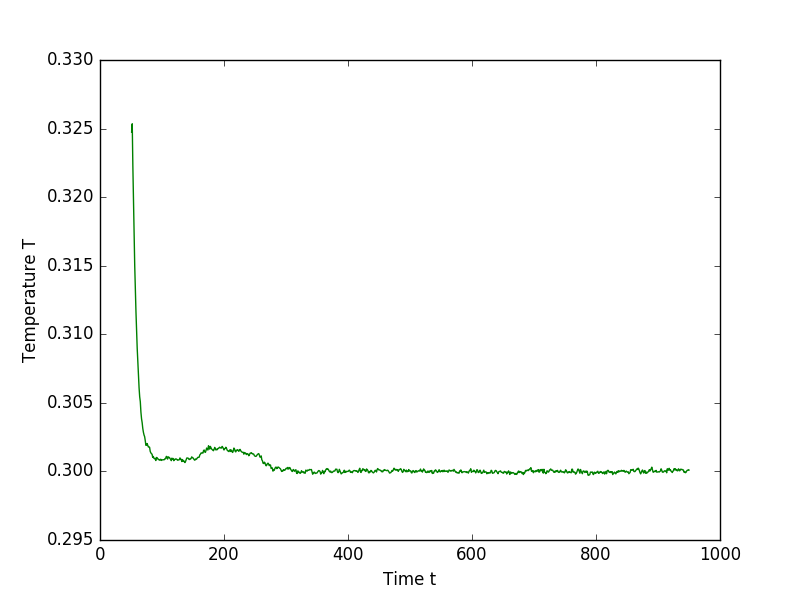
\includegraphics[width=\textwidth]{fig/avTemperature_T0d3_M100.png}
\end{subfigure}
\hfill
\begin{subfigure}{0.3\textwidth}
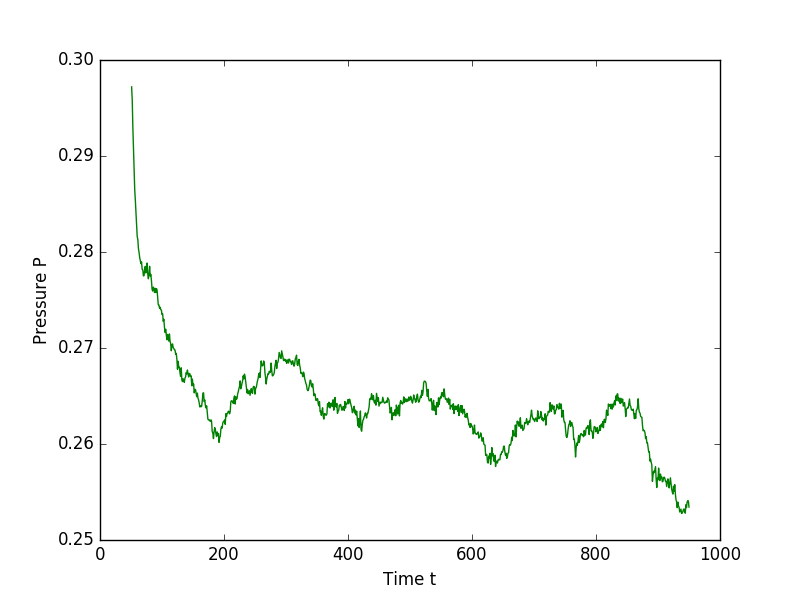
\includegraphics[width=\textwidth]{fig/avPressure_T0d3_M100.png}
\end{subfigure}
\hfill
\begin{subfigure}{0.3\textwidth}
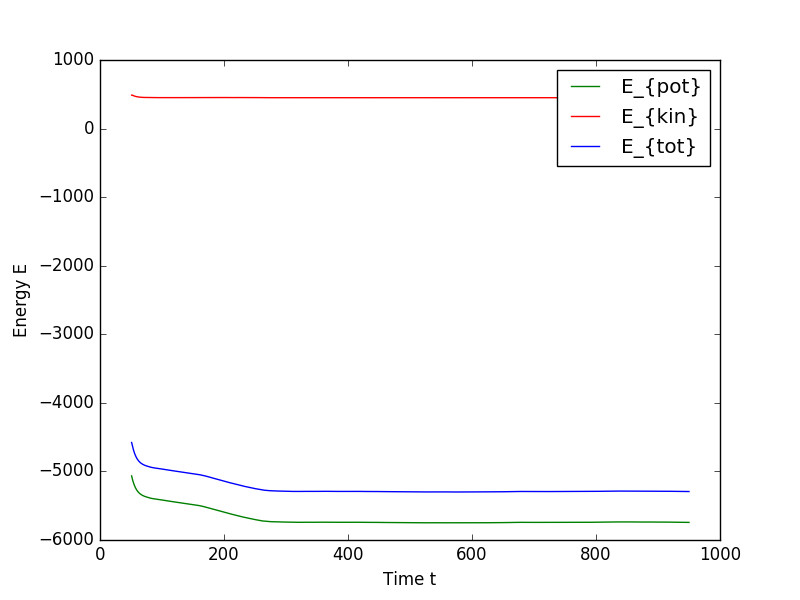
\includegraphics[width=\textwidth]{fig/avEnergies_T0d3_M100.png}
\end{subfigure}
\end{figure}

\begin{figure}[ht]
\begin{subfigure}{0.3\textwidth}
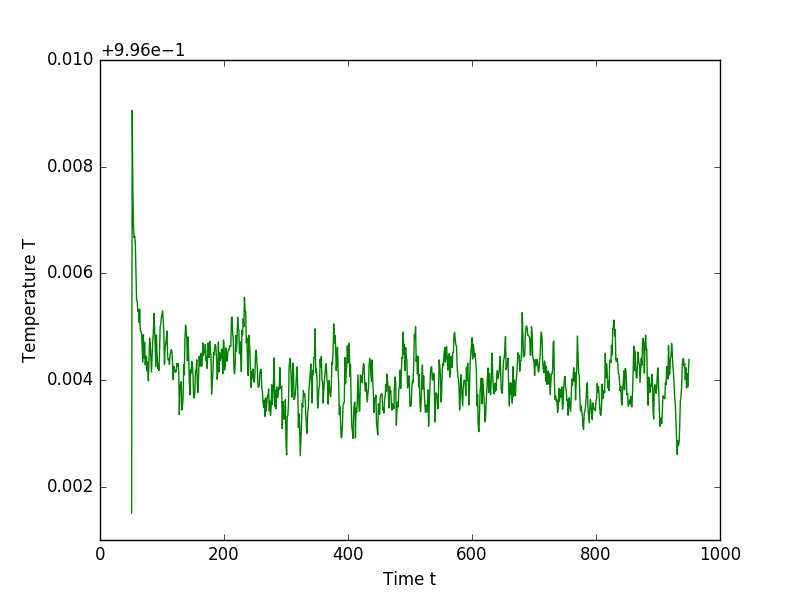
\includegraphics[width=\textwidth]{fig/avTemperature_T1d0_M100.png}
\end{subfigure}
\hfill
\begin{subfigure}{0.3\textwidth}
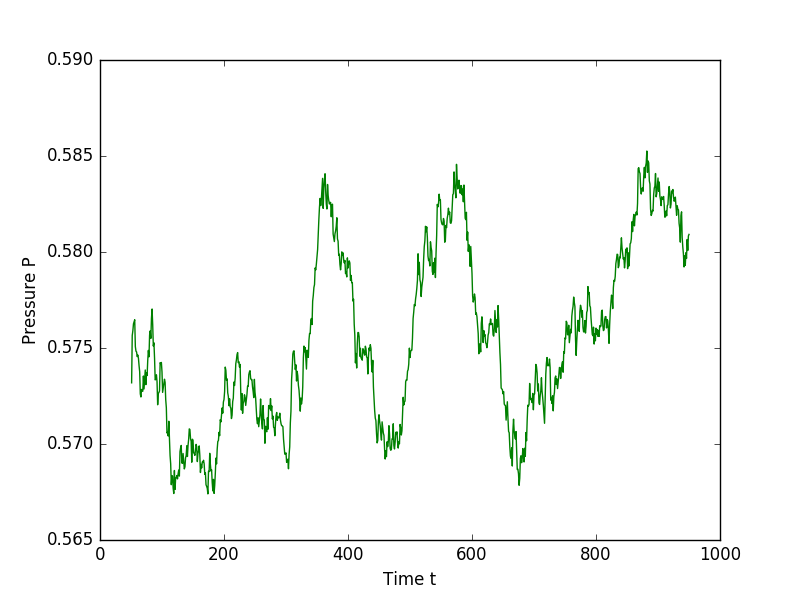
\includegraphics[width=\textwidth]{fig/avPressure_T1d0_M100.png}
\end{subfigure}
\hfill
\begin{subfigure}{0.3\textwidth}
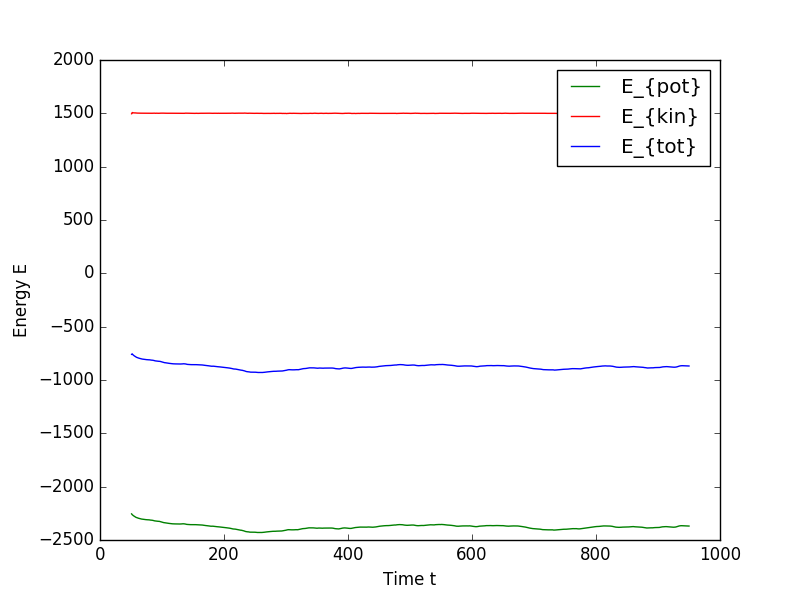
\includegraphics[width=\textwidth]{fig/avEnergies_T1d0_M100.png}
\end{subfigure}
\end{figure}

\begin{figure}[ht]
\begin{subfigure}{0.3\textwidth}
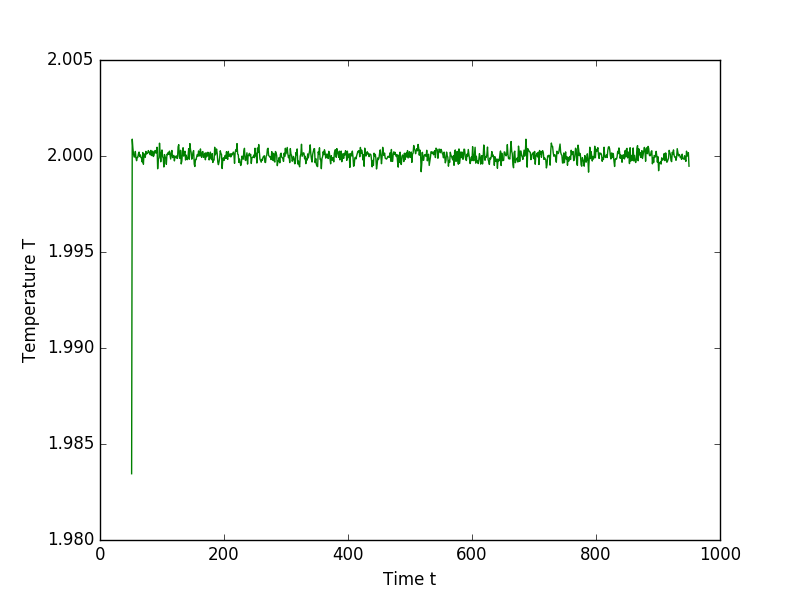
\includegraphics[width=\textwidth]{fig/avTemperature_T2d0_M100.png}
\end{subfigure}
\hfill
\begin{subfigure}{0.3\textwidth}
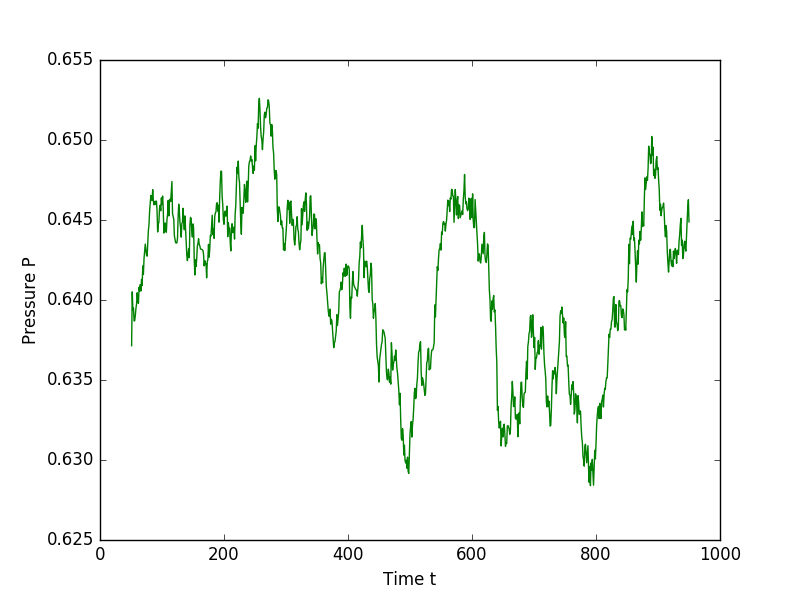
\includegraphics[width=\textwidth]{fig/avPressure_T2d0_M100.png}
\end{subfigure}
\hfill
\begin{subfigure}{0.3\textwidth}
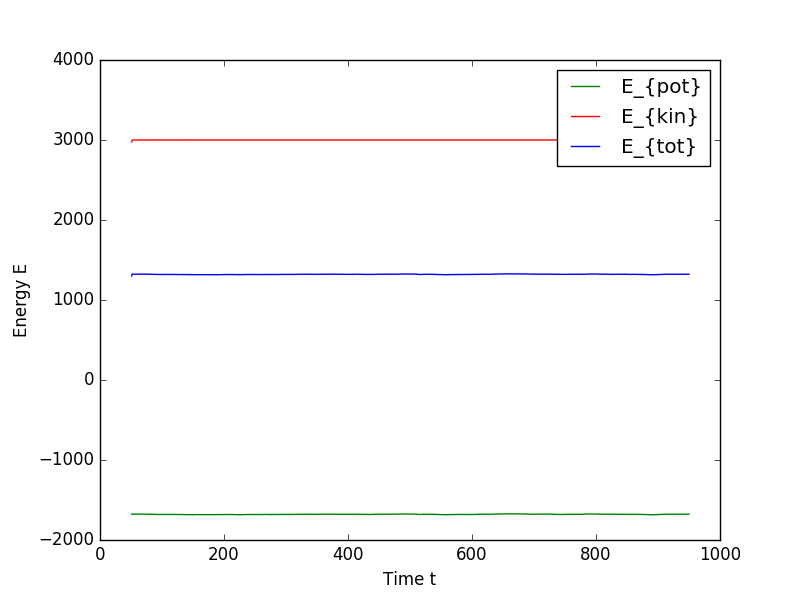
\includegraphics[width=\textwidth]{fig/avEnergies_T2d0_M100.png}
\end{subfigure}
\end{figure}
We can easily see the system reach the desired temperature and the energies reach equilibrium. The pressure is a bit harder to see as the fluctuations are so large and take large amounts of time.

